\section{Graph Neural Networks 2}
\subsection{Homogenous Graphs}
\(G = (V,E,)\)
\begin{table}[!h]
    \begin{tabular}{lr}
    Nodes     &  \(v_i \in V\)\\
    Edges      &  \((v_i,r,v_j) \in E\)
    \end{tabular}
\end{table}
Nodes and edges can have \textbf{attributes / features}.
Directed or undirected edges.

\subsection{Graphs}
Connectivity is specified by the \textbf{adjacency} matrix \textbf{A}.
\textbf{A} is often stored in a \textbf{sparse} formate.

\begin{figure}[!h]
    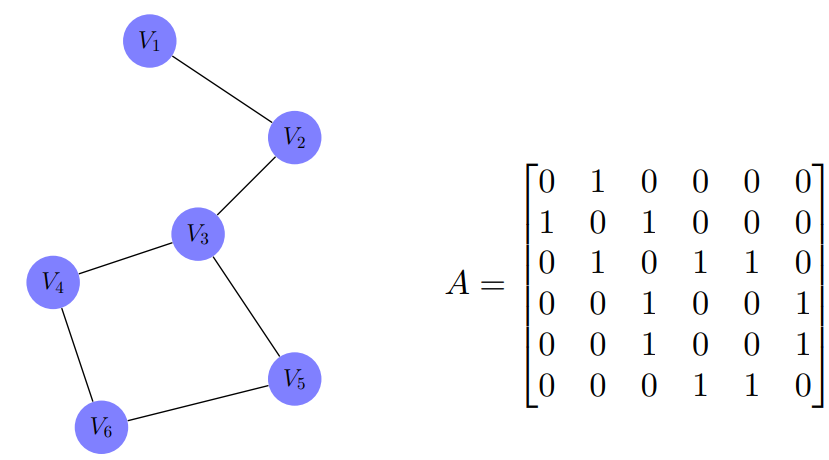
\includegraphics[width = \columnwidth]{figures/GraphNeuralNetworks2/SparseFormat.png}
\end{figure}

\subsection{Features}
Each node can contain a feature vector
\(x_i\) and each edge a feature vector \(e_{ij}\).
There might also be a global feature vector \(U\).

Many GNN approaches only use node features, so the graph is defined by \((A,X)\).
\begin{figure}[!h]
    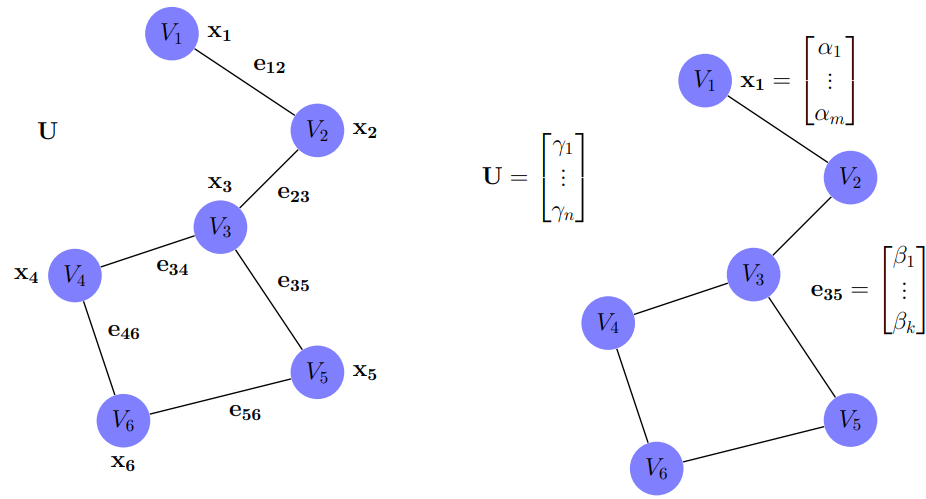
\includegraphics[width = \columnwidth]{figures/GraphNeuralNetworks2/Features.png}
\end{figure}

\subsection{GNNs: Idea}
Each layer of a GNN will \textbf{transform} the \textbf{transform} of the nodes and edges.
This is similar to an image going through the layers of a CNN.
\begin{figure}[!h]
    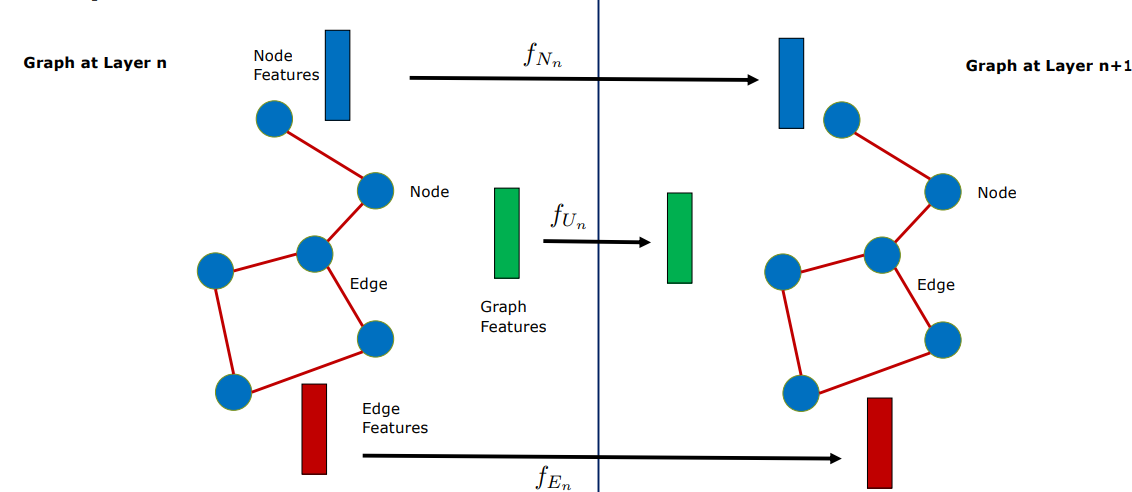
\includegraphics[width = \columnwidth]{figures/GraphNeuralNetworks2/GNNsIdea.png}
\end{figure}
\subsubsection{Feature Transformation}
\begin{itemize}
    \item The intermediate feature values for the nodes are commonly indicated by \(\mathbf{h}\) (similar to the hidden states in RNNs) and the output of the transformation is \(\mathbf{z}\).
    \item The dimension of the hidden values might change (similar to channels in CNNs).
\end{itemize}
\[
\mathbf{x} = 
\begin{bmatrix}
\dots \\
\dots \\
\dots
\end{bmatrix}
\longrightarrow
\mathbf{h}_1 = 
\begin{bmatrix}
\dots \\
\dots \\
\dots 
\end{bmatrix}
\longrightarrow
\hdots
\longrightarrow
\mathbf{h}_n = \mathbf{z} = 
\begin{bmatrix}
\dots \\
\dots \\
\dots
\end{bmatrix}
\]

\subsection{Graph Convolutions by Spectral Methods}
Convolutions turn into element-wise multiplications in the spectral domain by the Fourier Transform.
After the convolutions, the signal can be turned back using the inverse Fourier Transform.

The Graph Fourier Transform can be calculated using the Eigenvalues of the Laplacian:
\[
L = U\Lambda U^T \qquad \Lambda = \text{diag}(\left[\lambda_0,\lambda_1,\dots,\lambda_n\right])
\]
Convolution with learnable function g:
\[
g \ast x = F^{-1}(F(g)\times F(x)) = U(U^Tg\times U^Tx)
\]
\subsection{Some graph math for calculating GNNs}
\begin{itemize}
    \item The \textbf{degree} of a node is the number of its direct neighbours.
    \item If \(mathbf{A}\) is given, the degree can be calculated by summing the nodes
    \item It is usually written as a diagonal matrix \(mathbf{D}\)
\end{itemize}
\begin{figure}[!h]
    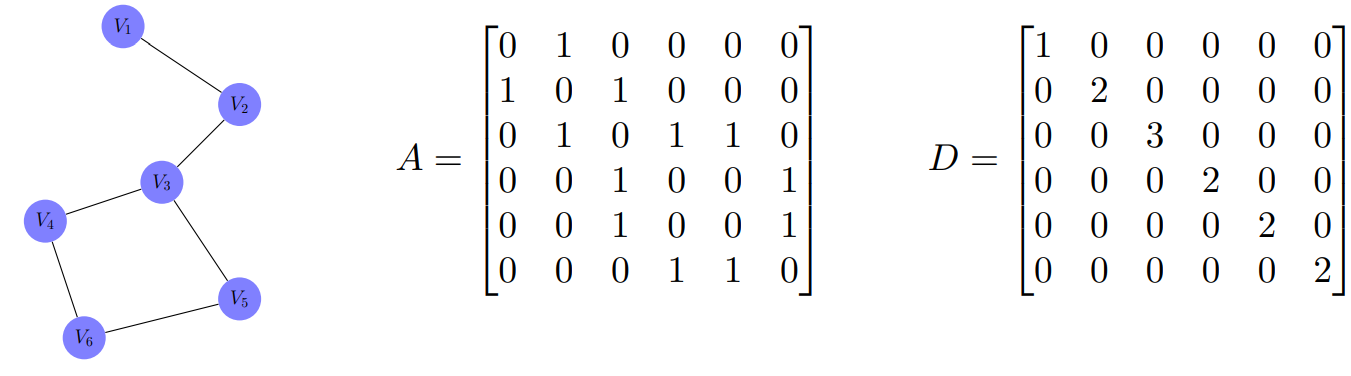
\includegraphics[width = \columnwidth]{figures/GraphNeuralNetworks2/MathForGNNS.png}
\end{figure}

\subsubsection{Graph Laplacian}
\begin{table}[!h]
    \begin{tabular}{lr}
    Graph Laplacian    &  \(L = D - A\)\\
    Edges with relation types     &  \(L = 
    \begin{bmatrix}
      1  & -1 &  0 &  0 &  0 &  0 \\
     -1  &  2 & -1 &  0 &  0 &  0 \\
      0  & -1 &  3 & -1 & -1 &  0 \\
      0  &  0 & -1 &  2 &  0 & -1 \\
      0  &  0 & -1 &  0 &  2 & -1 \\
      0  &  0 &  0 & -1 & -1 &  2 \\
    \end{bmatrix}\)\\
    Normalized Laplacian    & \(L = I-D^{-\frac{1}{2}}AD^{-\frac{1}{2}}\)
    \end{tabular}
\end{table}
\subsubsection{Spectral Methods}
\begin{itemize}
    \item The filter in spectral networks is applied over the entire (connected) graph, so there is no locality
    \item Caculation of the eigenvalues is inefficient
    \item ChebNets use Chebyshew Polynomials to define a convolution that uses only a k-hop neghborhood of a node
    \item Graph Convolutional Networks (GCN) use \(k = 1\)
\end{itemize}
\subsection{Graph Convolutional Networks (GCN)}
\begin{itemize}
    \item Enforce self-connection by using\[
    \tilde{A} = A + I_n \qquad \tilde{D}_{ij} = \sum_{j}^{}\tilde{A}_{ij}
    \]
    \item and calculate the normalized Laplacian, which now has eigenvalues in \([0 \dots 1]\) (no exploding gradients)
    \[
    L_{norm} = \tilde{D}^{-\frac{1}{2}}\tilde{A}\tilde{D}^{-\frac{1}{2}}
    \]
    \item The update rule then becomes:
    \[
    H^{l+1} = \sigma(\tilde{D}^{-\frac{1}{2}}\tilde{A}\tilde{D}^{-\frac{1}{2}}H^{(l)}W^{(l)})
    \]
\end{itemize}
The update rule can be written in the spatial domain as 
\[
h_i^{(l)} = \sigma\left(\sum_{i \in N_j}c_{ij}Wh-j\right)
\]
where
\[
c{ij} = \frac{1}{\sqrt{|N_i||N_j|}}
\]
and \(|N_i||N_j|\) are the sizes of the node neighborhood.
\begin{figure}[!h]
    \centering
    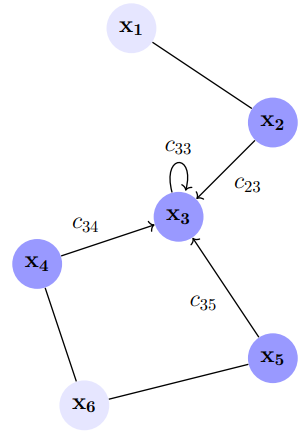
\includegraphics[width = 0.3\columnwidth]{figures/GraphNeuralNetworks2/GCN.png}
\end{figure}
\subsubsection{Node Classification}
\begin{itemize}
    \item For node classification, a classifier can be added that uses the output \(\mathbf{z}\) of a node for classification.
    \item Node classification can be \textbf{semi-supevised}: The GNN is trained on the graph which contains some labelled node and then used to predict the classes of the remaining nodes.
\end{itemize}
\subsubsection{Graph Convolutional Networks: Loss}
Loss for semi-supervised learning (node classification) in the spectral formulation
\[
    \mathcal{L} = \mathcal{L}_0 + \lambda \mathcal{L}_{reg} \quad \mathcal{L}_{reg} = \sum_{i,j}A_{ij}||f(X_i)- f(X_j)||^2 = f(X)^T\nabla f(x)
\]
\(\mathcal{L}_0\) is the supervised loss with respect to the labelled parts of the graph, \(X\) are the node features and \(f\) a Neural Network.

\subsection{Semi-supervised node classification with GCN: Example}
\subsubsection{Node Embeddings}
\begin{itemize}
    \item Node embeddings map a node to a feature vector \(z\)
    \item Similarity in the embedding space should approximate similarity in the graph
    \item This is an \textbf{unsupervised} task
\end{itemize}
\subsubsection*{Node Embeddings: Variational Graph Auto Encoder (VGAE)}
Use a Variational Auto Encoder (VAE) to encode and decode a graph:
\begin{itemize}
    \item The encoder calculates an embedding or \textbf{latent variable z}
    \item The decoder calculates the graph from z by predicting the \textbf{adjacency matrix A}
\end{itemize}
For a simple auto encoder, this can be achieved by
\[
\hat{\mathbf{A}} = \sigma(\mathbf{Z}\mathbf{Z}^T), \text{with} \mathbf{Z} = GCN(\mathbf{X},\mathbf{A})
\]
I.e. the encoder is a graph convolutional network, the decoder a simple inner product.
\begin{itemize}
    \item (Variational Auto Encoder use a more complicated loss function to ensure z is Gaussian distributed)
    \item VGA can be used for \textbf{link prediction}
\end{itemize}

\subsubsection{Spacial Methods}
Spetial methods define convolutions directly on the graph, based on the topology.
Usually:
\begin{itemize}
    \item The features vectors are transformed
    \item They are aggregated in a permutation-invariant function
    \item The feature vector of each node is updated from its current value and the aggregated neighborhood representation
\end{itemize}
Popular methods:
\begin{itemize}
    \item GraphSAGE
    \item Message Passing Neural Network (MPNN) 
\end{itemize}
\subsubsection*{GraphSAGE}
Update node features as
\[
\mathbf{x}_i' = \mathbf{W}_1\mathbf{x}_i + \mathbf{W}_2 \times \text{mean}_{j \in \mathcal{N}(i)}\mathbf{x}_j
\]

with (optionally) first projecting \(x_j\)
\[
\mathbf{x}_j \leftarrow \sigma (\mathbf{W}_3 \mathbf{x}_j + \mathbf{b})
\]
For training on a number of input nodes (for a minibatch), their neighborhood is sampled as needed for computation.
\begin{figure}[!h]
    \centering
    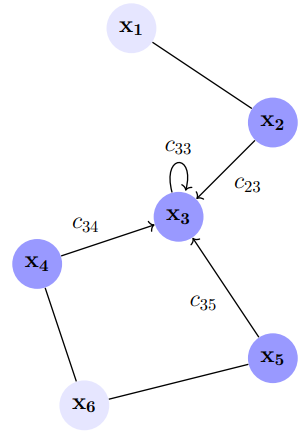
\includegraphics[width = 0.3\columnwidth]{figures/GraphNeuralNetworks2/GCN.png}
\end{figure}
Possible aggregation functions are:
\begin{itemize}
    \item Mean:
    \[
        \mathbf{h}_v^k \leftarrow (\mathbf{W} \cdot \text{MEAN}(\left\{\mathbf{h}_v^{k-1}\right\}\cup\left\{\mathbf{h}_u^{k-1},\forall u \in \mathcal{N}(v)\right\}))
    \]
    \item LSTM: LSTM cell with random permutation of node's neighbors
    \item Pooling:
    \[
        \text{AGGREGATE}_k^{pool} = \max\left(\left\{\sigma(\mathbf{W}_{pool}\mathbf{h}_{ui}^k + \mathbf{b}),\forall u_i \in \mathcal{N}(v)\right\}\right)
    \]
    \item Experiments show that LSTM and pooling perform best.
\end{itemize}


\subsection{Message Passing Neural Networks (MPNN)}
\begin{itemize}
    \item Message \(m_{ij}\) can be sent across edges between nodes \(V_i\) and \(V_j\) and are computed using a message function (small MLP).
    \[
    m_{ij} = f_e(h_i,h_j,e_{ij})
    \]
    \item Messages are aggregated using a permutation-invariant function (sum, mean, max, etc.)
    \item The aggregated message is combined with the current node features and updated using another function
    \[
    h_i = f_v(h_i,\sum_{j \in N_i}m_{ji})
    \]
\end{itemize}
\begin{figure}[!h]
    \centering
    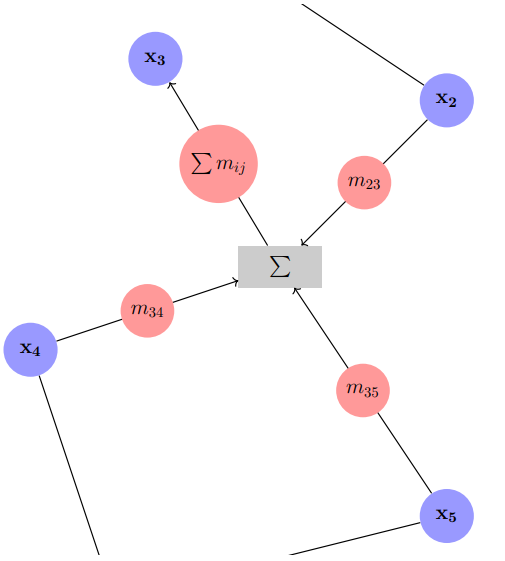
\includegraphics[width = 0.3\columnwidth]{figures/GraphNeuralNetworks2/MessagePassing1.png}
    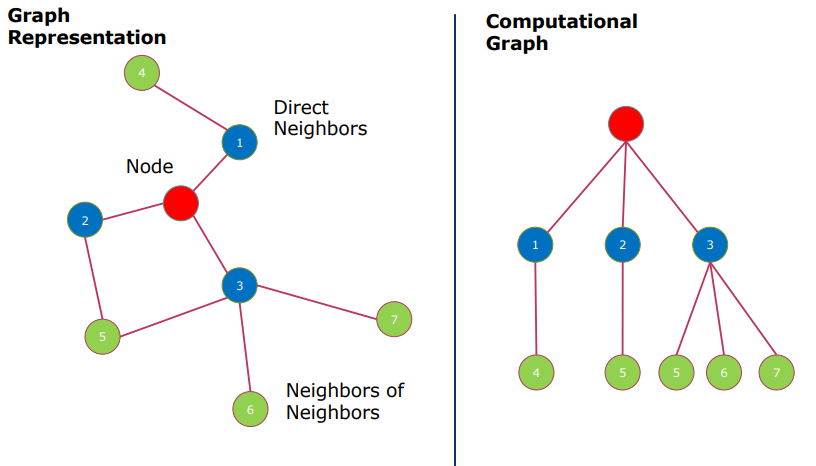
\includegraphics[width = 0.65\columnwidth]{figures/GraphNeuralNetworks2/MessagePassing2.png}
\end{figure}

\subsection{Graph Attention Networks}
In GCNs features from neighboring nodes are weighted by their degree
\[
h_i^{(i)} = \sigma \left(\sum_{i \in N_j}\frac{1}{\sqrt{|N_i||N_j|}}Wh_j\right)
\]
these are statistically defined from the graph and might not always be beneficial.
\begin{itemize}
    \item Simple, spatial convolutions can also be calculated without these weights, or
    \item The weights could be calculated from the features to see which nodes are more important
    \item Calculate attention scores on a trainable linear transform of the node featues for the nodes \(j \in \mathcal{N}_i\) neighbors:
    \[
    e_{ij} = a(\mathbf{Wh}_i,\mathbf{Wh}_j)\\
    \alpha_{ij} = softmax_j(e_{ij}) = \frac{\text{exp}(e_{ij})}{\sum_{k\in\mathcal{N}_i}\text{exp}(e_{ik})}
    \]
     \item The attention mechanism here is a single layer MLP (instead of the scalar dot product)
\end{itemize} 
The new features of a node are then calculated as 
\[
\vec{h}_i' = \sigma \left(\sum_{j \in \mathcal{N}_i} \alpha_{ij}\mathbf{W}\vec{h}_j\right)
\]
additionally Multi-headed Attetion is used
\begin{figure}[h!]
    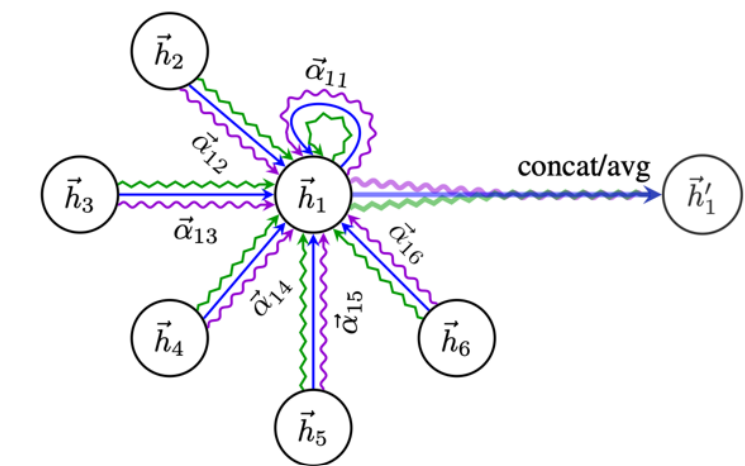
\includegraphics[width = 0.5\columnwidth]{figures/GraphNeuralNetworks2/GraphAttentionNetworks.png}
\end{figure}

\subsection{Graph Classification}
\begin{itemize}
    \item For graph classification, often the resulting output features \(\mathbf{z}\) of the nodes are used and combined in a so-called \textbf{readout} operation
    \item This results in a single vector for the graph, which is then used as input for classification
    \item Graph Classification is usually \textbf{supervised learning}, the GNN is trained on many different graphs, and then applied to a new graph
\end{itemize}

\subsection{Conclusion}
\begin{itemize}
    \item GNNs are an evolving and active field
    \item There are many different approaches and no cnosensus yet
    \item Some approaches are coupled with their applications (node/graph level tasks \& unsupervised, semi-supervised and supervised settings)
    \item Message passing provides a conveniant way to describe many variants of GNNs
\end{itemize}